% arara: pdflatex
% !arara: indent: {overwrite: yes}
\documentclass[12pt]{article}
\usepackage[margin=.5cm]{geometry}
\usepackage{ifthen}
\usepackage{tikz}
\usetikzlibrary{matrix}
\usetikzlibrary{shapes}
\usetikzlibrary{decorations}
%\usetikzlibrary{decorations.shapes}
%\usetikzlibrary{decorations.pathmorphing}
\usetikzlibrary{decorations.markings}

\newcounter{totalpoints}
\newcommand{\points}[1]{%
\ifthenelse{\equal{#1}{bronze}}{10\addtocounter{totalpoints}{10}}{}%
\ifthenelse{\equal{#1}{silver}}{20\addtocounter{totalpoints}{20}}{}%
\ifthenelse{\equal{#1}{gold}}{30\addtocounter{totalpoints}{30}}{}%
}
\tikzset{
	empty/.style={
		draw=gray,
		star,
		anchor=center,
		scale=2,
	},
	badge/.style={
		scale=1.2,
		text=white,
		fill=black!70,
		rounded corners=1ex,
		text width=5cm,
		minimum width=3cm,
		minimum height=1.1cm,
		align=right,
		font=\bfseries,
            %    append after command={
            %    [very thick,shorten >=0.2bp, shorten <=0.2bp]
            %                (\tikzlastnode.west)edge(\tikzlastnode.east)coordinate[midway](cmh)
            %    },
		%        postaction={\node at (current bounding box.west){f}},
		decoration={
			markings,% switch on markings
        %          %mark = at position 1 with {\arrow{>}}
%       %           mark = at position 1 with {\arrow{>}}
       %mark = at position 0.2 with {\node[draw, circle, fill = white, inner sep = .05cm, scale = .75] {2};},
                %          mark = at position 0 with {\filldraw[black] circle (.05cm);}, 
			 mark=% actually add a mark
			 at position 0cm
			 with
             {%\node[draw, circle,fill=red,] {f};}%
                \coordinate (cmh) at (157pt,22pt);
			 	%\draw[fill=#1] (160pt,18pt) circle (.9ex);
                \node[
                draw=white,
                double,
                fill=#1,
                align=center, 
                circle,
                text=black,
                inner sep=0pt,
                scale=.15,] at (cmh) {\resizebox{2.5cm}{!}{\points{#1}}};
			 }
		},
		postaction=decorate,
	},
	badge/.default=bronze,
	description/.style={
		fill=none,
		draw=none,
		text=black,
		font=\itshape,
	},
}


\pagestyle{empty}
\begin{document}


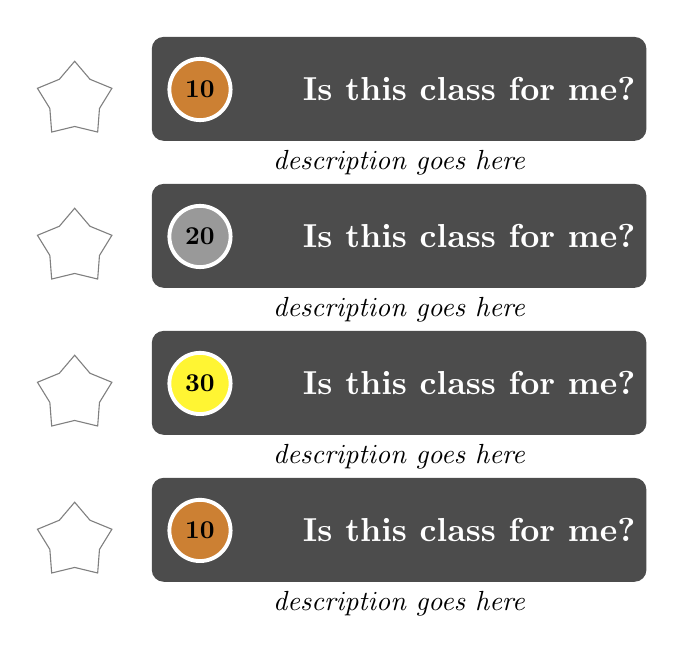
\begin{tikzpicture}
	\colorlet{bronze}{brown!80!orange}
	\colorlet{silver}{gray!80!white}
	\colorlet{gold}{yellow!80!white}
	\matrix[matrix of nodes,
		nodes in empty cells,
		column sep=.5cm,
		execute at empty cell={\node[empty]{};},
		%column 2/.style={nodes={badge}},
		every even row/.style={
			nodes={description},
		},
	]{
		%* \begin{tabular}
		   & |[badge]| Is this class for me?    \\
		{} & description goes here                  \\
		   & |[badge=silver]|Is this class for me?  \\
		{} & description goes here                  \\
		   & |[badge=gold]|Is this class for me?    \\
		{} & description goes here                  \\
		   & |[badge=bronze]| Is this class for me? \\
		{} & description goes here                  \\
		};
		%* \end{tabular}
	\end{tikzpicture}
\end{document}

% old attempt
% old attempt
% old attempt
\begin{tikzpicture}
	\matrix[matrix of nodes,
		nodes in empty cells,
		execute at empty cell={\node[empty]{};},
		column 2/.style={nodes={badge}},
		column 3/.style={nodes={font=\itshape}},
	]{%
		& Is this class for me? & description goes here\\
		& Is this class for me? & description goes here\\
		& Is this class for me? & description goes here\\
		& Is this class for me? & description goes here\\
		& Is this class for me? & description goes here\\
	};
\end{tikzpicture}
